\section{Radioactive Byproducts of Proton and Neuton Irradiation and Associated Dangers}


\subsection{Radioactivity, Absorbed Dose, Dose Equivalent and Exposure}

There is a distinction between how radioactive a source is and how much radiation is absorbed by an organic due to that source.  
There are different measures of radioactivity and it's effects, and they may be summarised very briefly as follows:

\begin{itemize}
\item Radioactivity of a source - decay events per second (Bq)  (also measured in Curie, $3.7 x 10^10$ decays per second)
\item Absorbed dose of any target - energy absorbed per unit mass (Gy) (equivalent of Joules per Kilo)
\item Equivalent dose absorbed by tissue/organ - type of radiation is important (Si)
\item Effective dose on tissue/organ - how the equivalent dose affects the specific tissue/organ (Si)
\end{itemize}

One joule of ionising radiation absorbed by a person may not seem a lot of energy, but the average annual doses are so small they are measured in millisieverts per year.  A dose of just 5 Sieverts is enough to kill 50% of people within 1 month. 

\begin{table}[h]
\begin{center}
\begin{tabular}{c c}
\hline
Exposure & Dose (mSv) \\
\hline \\
Dental X-ray & 0.005 \\
Chest X-ray & 0.02 \\
UK average annual dose &  2.7 \\
Whole bodt CT scan & 10 \\
Nuclear industry employee annual exposure & 20 \\
Acute radiation effects & 1,000 \\
50% lethal dose within 1 month & 5,000 \\
\end{tabular}
\end{center}
\caption{DFT Settings}
\end{table}



In an MCNP5 simulated neutron flux environment, with a thermal flux of $2.5 \times 10^7 n/cm^2 s$ a stainless steel cylinder, 20mm diameter and 70mm irradiated for 10 hours\cite{radionuclides}.  After 10 minutes cooling, it was calculated to have an activity of over $1.0e7$ Bq, predominantly due to the creation of Mn\textsuperscript{56}.  

The activity in this work seems slightly.  The maximum cross section of Mn\textsuperscript{55} (n, $\gamma$) Mn\textsuperscript{56} is 2.0 barns and the estimated reaction rate at this flux is just over $2.0e^6$.  As the half life of Mn\textsuperscript{55} is short compared to the irradiation time (2.5 hours) the maximum number of Mn\textsuperscript{55} atoms are created, with the creation rate equalling the decay rate.

A simple neutron activation code was developed, which will be discussed in more detail in this work, and the predicted Mn\textsuperscript{55} activity vs time was calculated.

\begin{figure}
  \begin{center}
    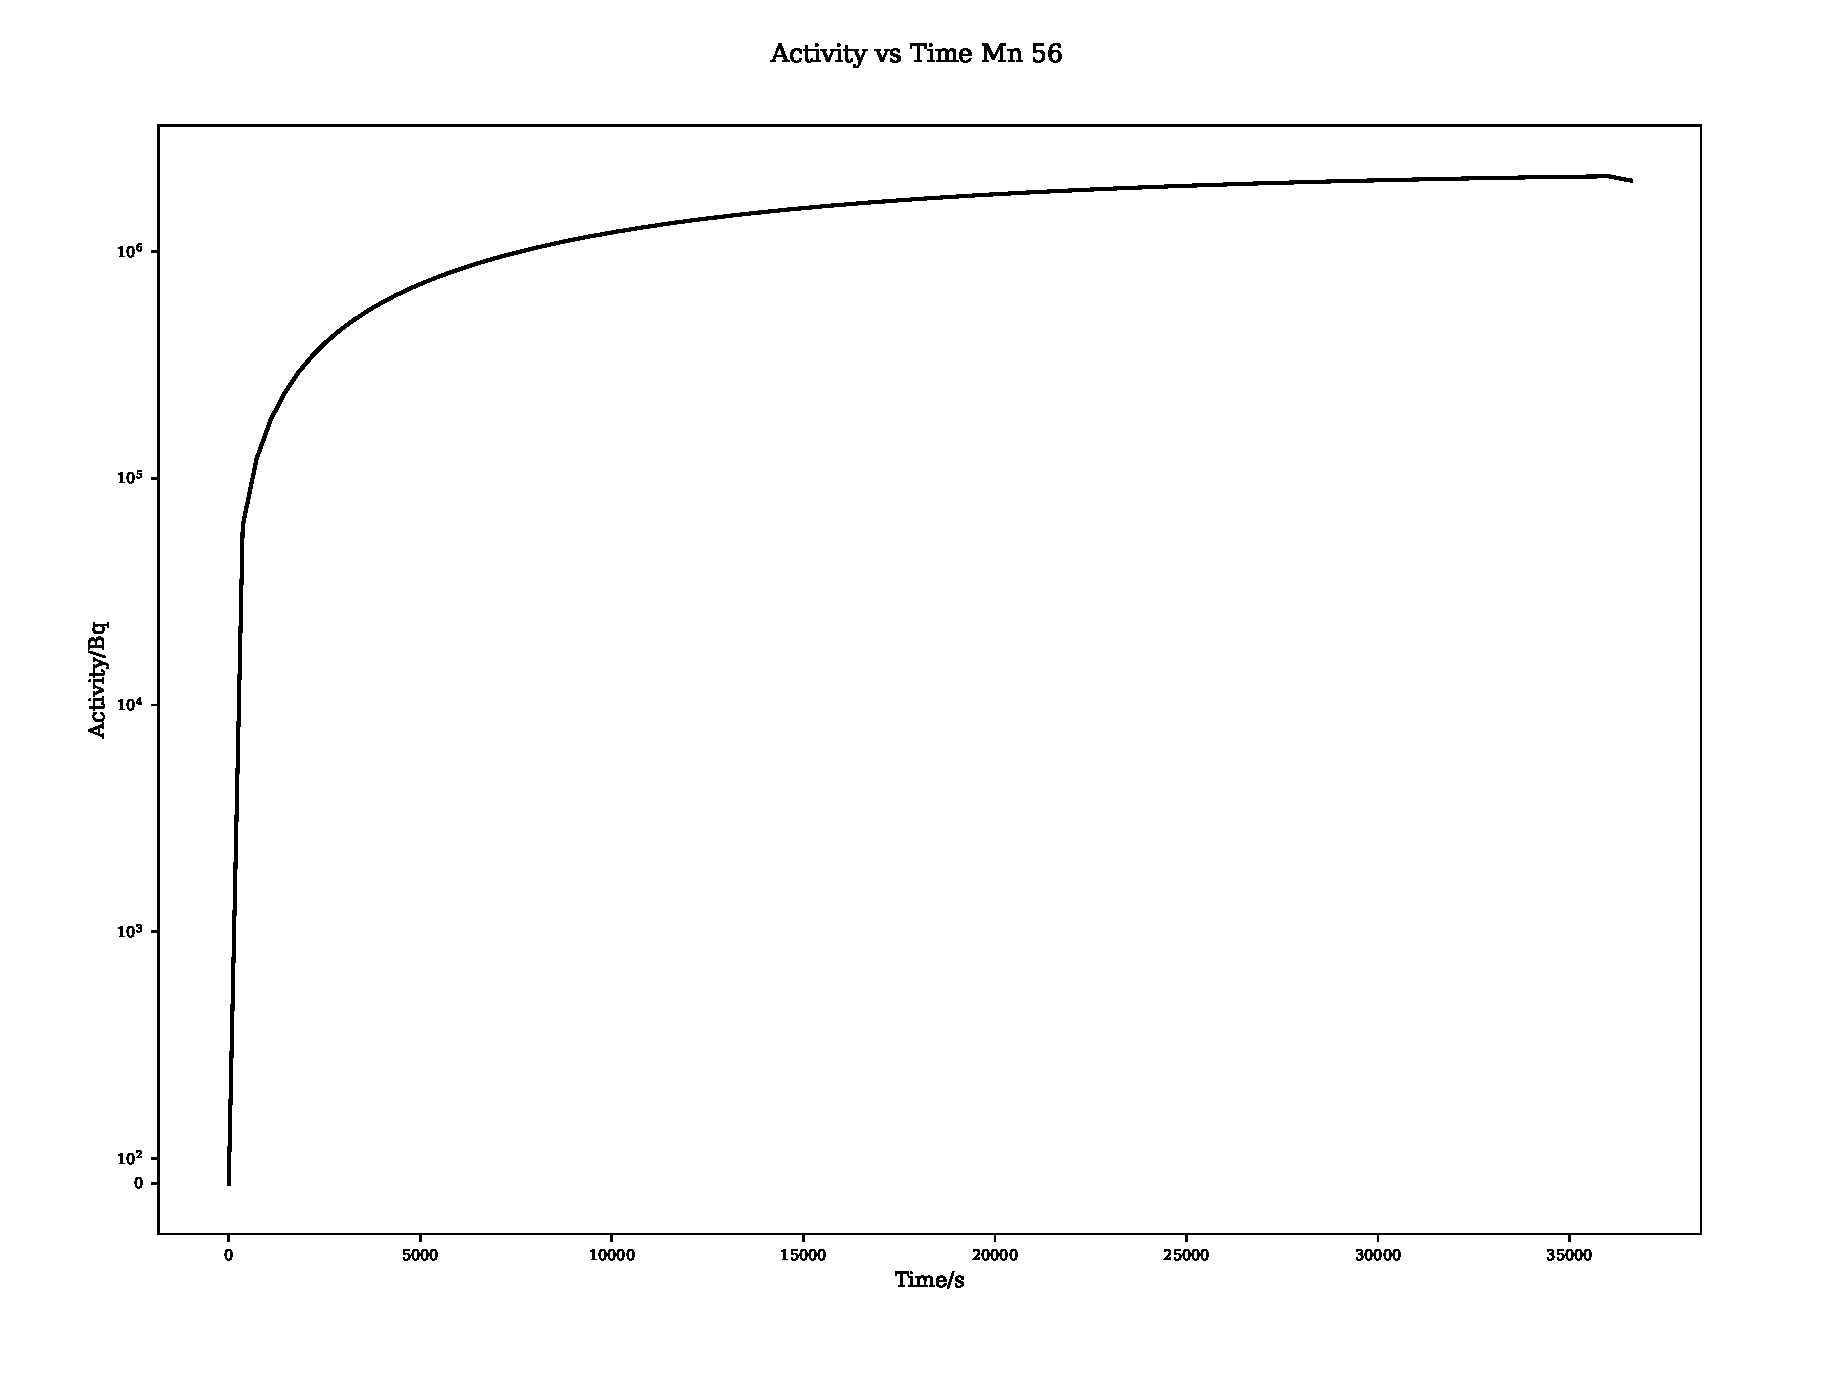
\includegraphics[width=15.0cm]{chapters/background_radiation_effects_and_transport/neutron_plots/1/25_Mn_56_activity.eps}
    \captionsetup{font={it}}
    \caption{Mn 56 Activity}
    \label{fig:mn_56_activity}
  \end{center}
\end{figure}

The overall gamma dose, for 1 minute of exposure to an 80kg person standing 2m from the source was also calculated.

\begin{figure}
  \begin{center}
    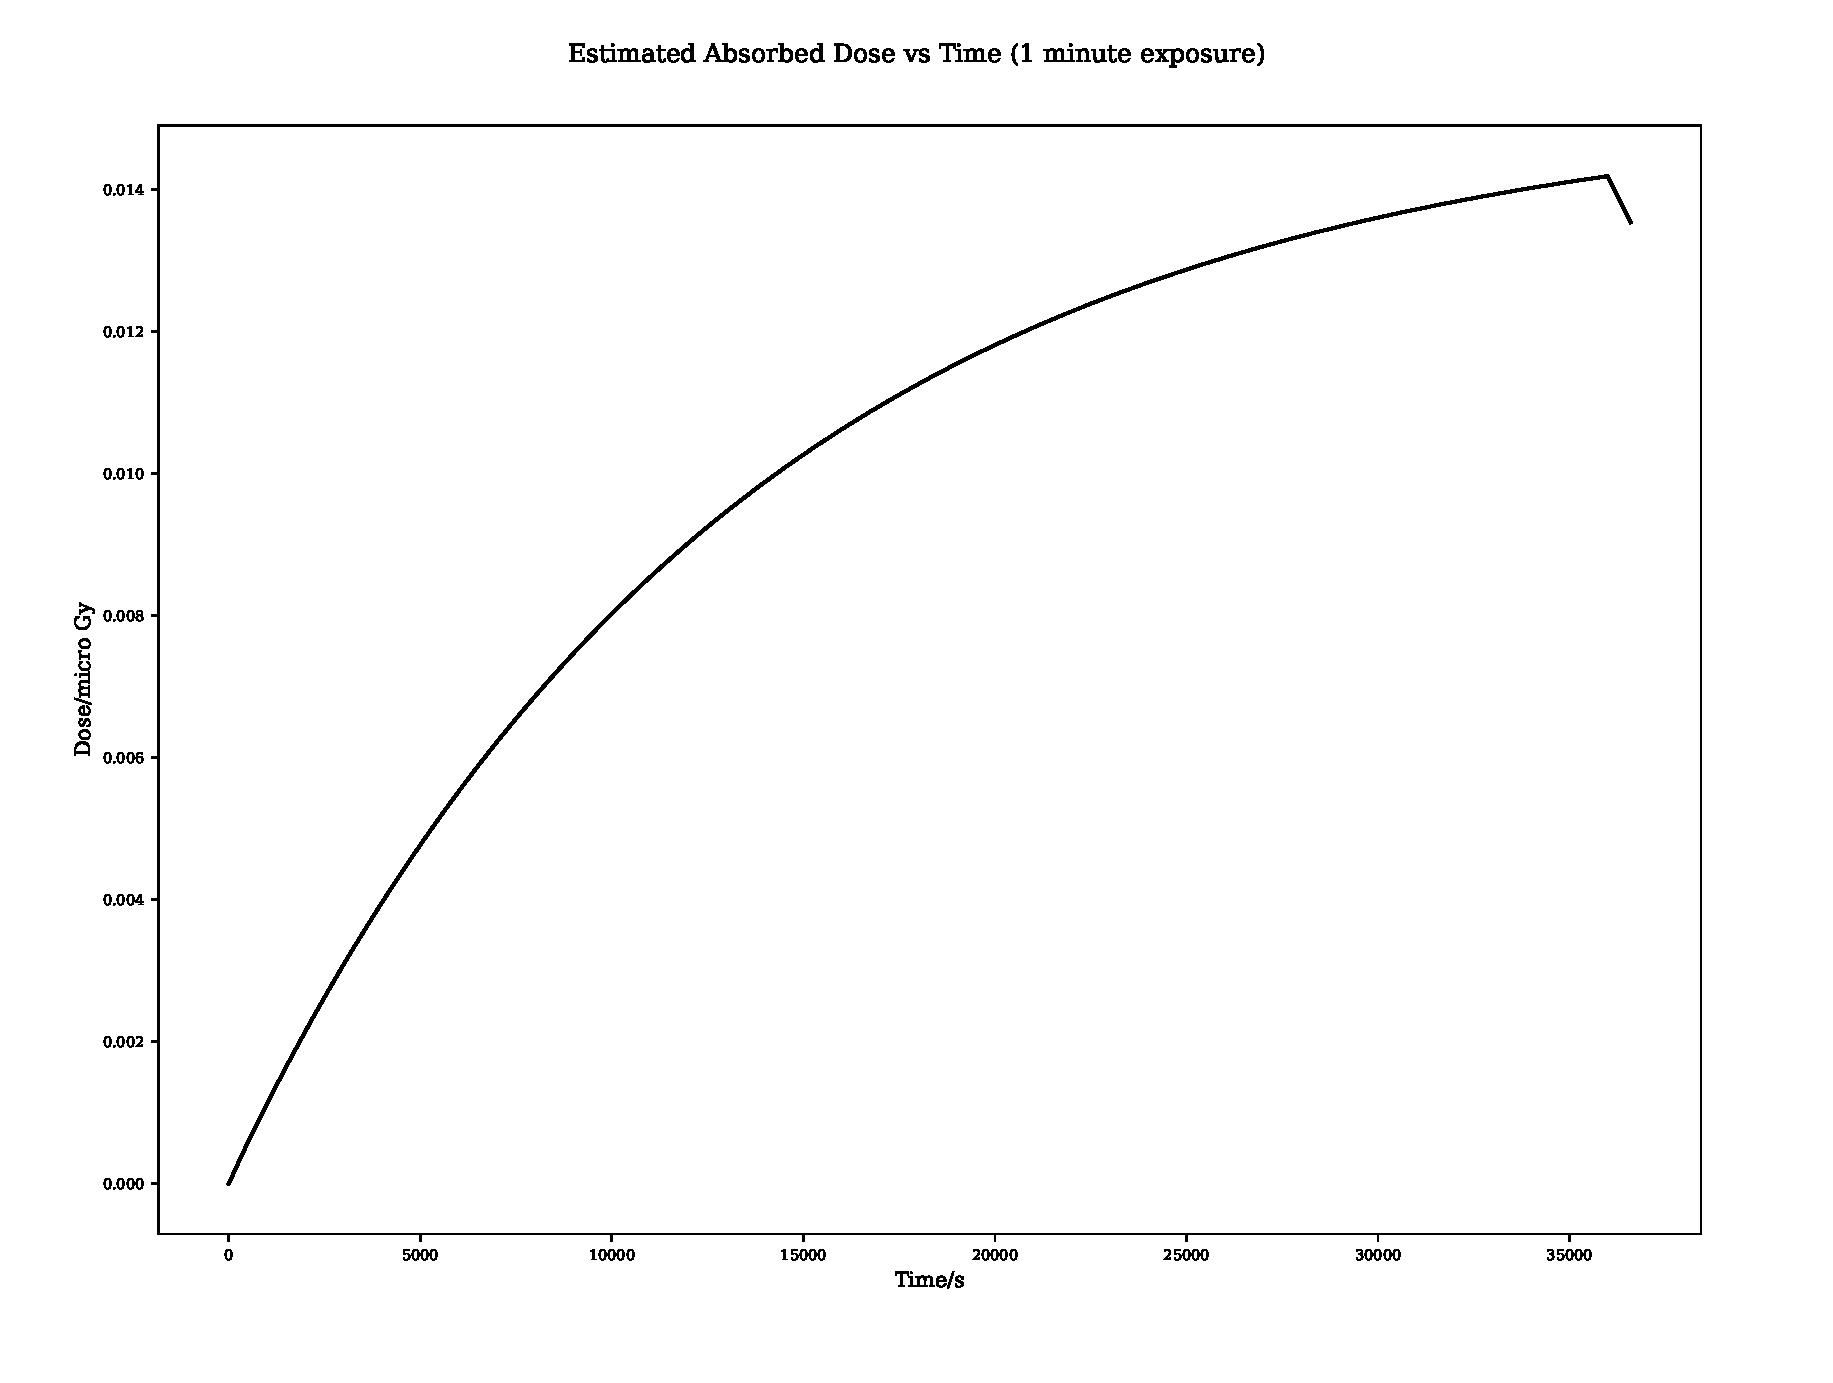
\includegraphics[width=15.0cm]{chapters/background_radiation_effects_and_transport/neutron_plots/1/gamma_dose.eps}
    \captionsetup{font={it}}
    \caption{Steel Irradiation Gamma Dose 2.5e7 Neutrons per cmsquared per second}
    \label{fig:ga_vs_sim_512_2}
  \end{center}
\end{figure}

The flux in the within the flux trap of the HFIR is much higher, with high energy neutrons having a flus of $1.0e14$ neutrons per cmsquared per second.  

\begin{figure}
  \begin{center}
    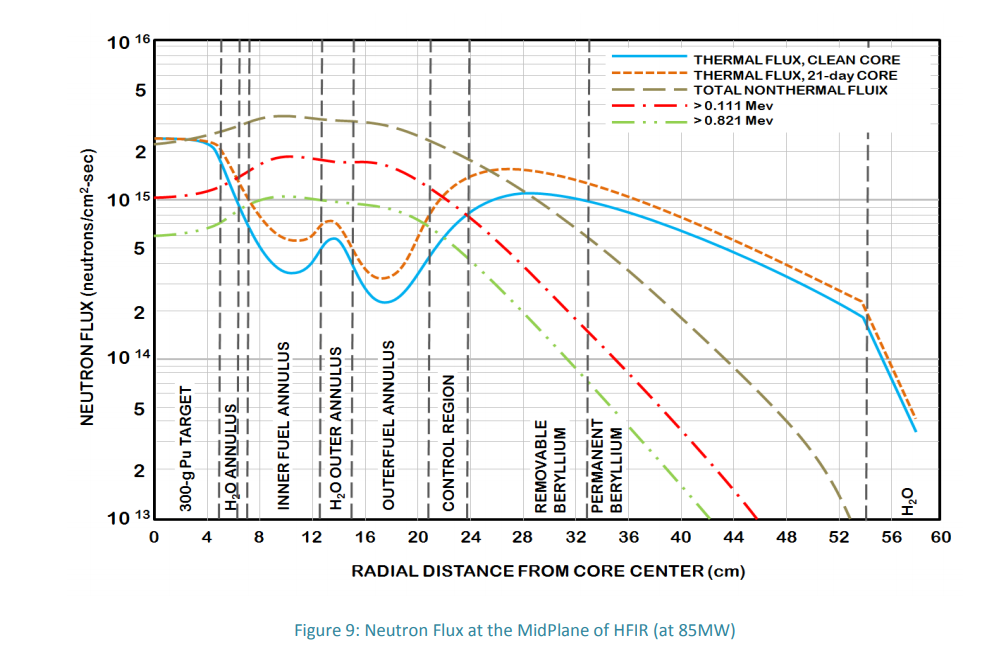
\includegraphics[width=15.0cm]{chapters/background_radiation_effects_and_transport/images/HFIR_neutron_spectra_guide.png}
    \captionsetup{font={it}}
    \caption{High Flux Isotope Reactor Neutron Flux}
    \label{fig:ga_vs_sim_512_2}
  \end{center}
\end{figure}

A second calculation was performed for this increased flux, also irradiated over 10 hours.  The overall dose per minute was much higher, between 40 and 50 milligrey per minute over the first hour of cooling.  

\begin{figure}
  \begin{center}
    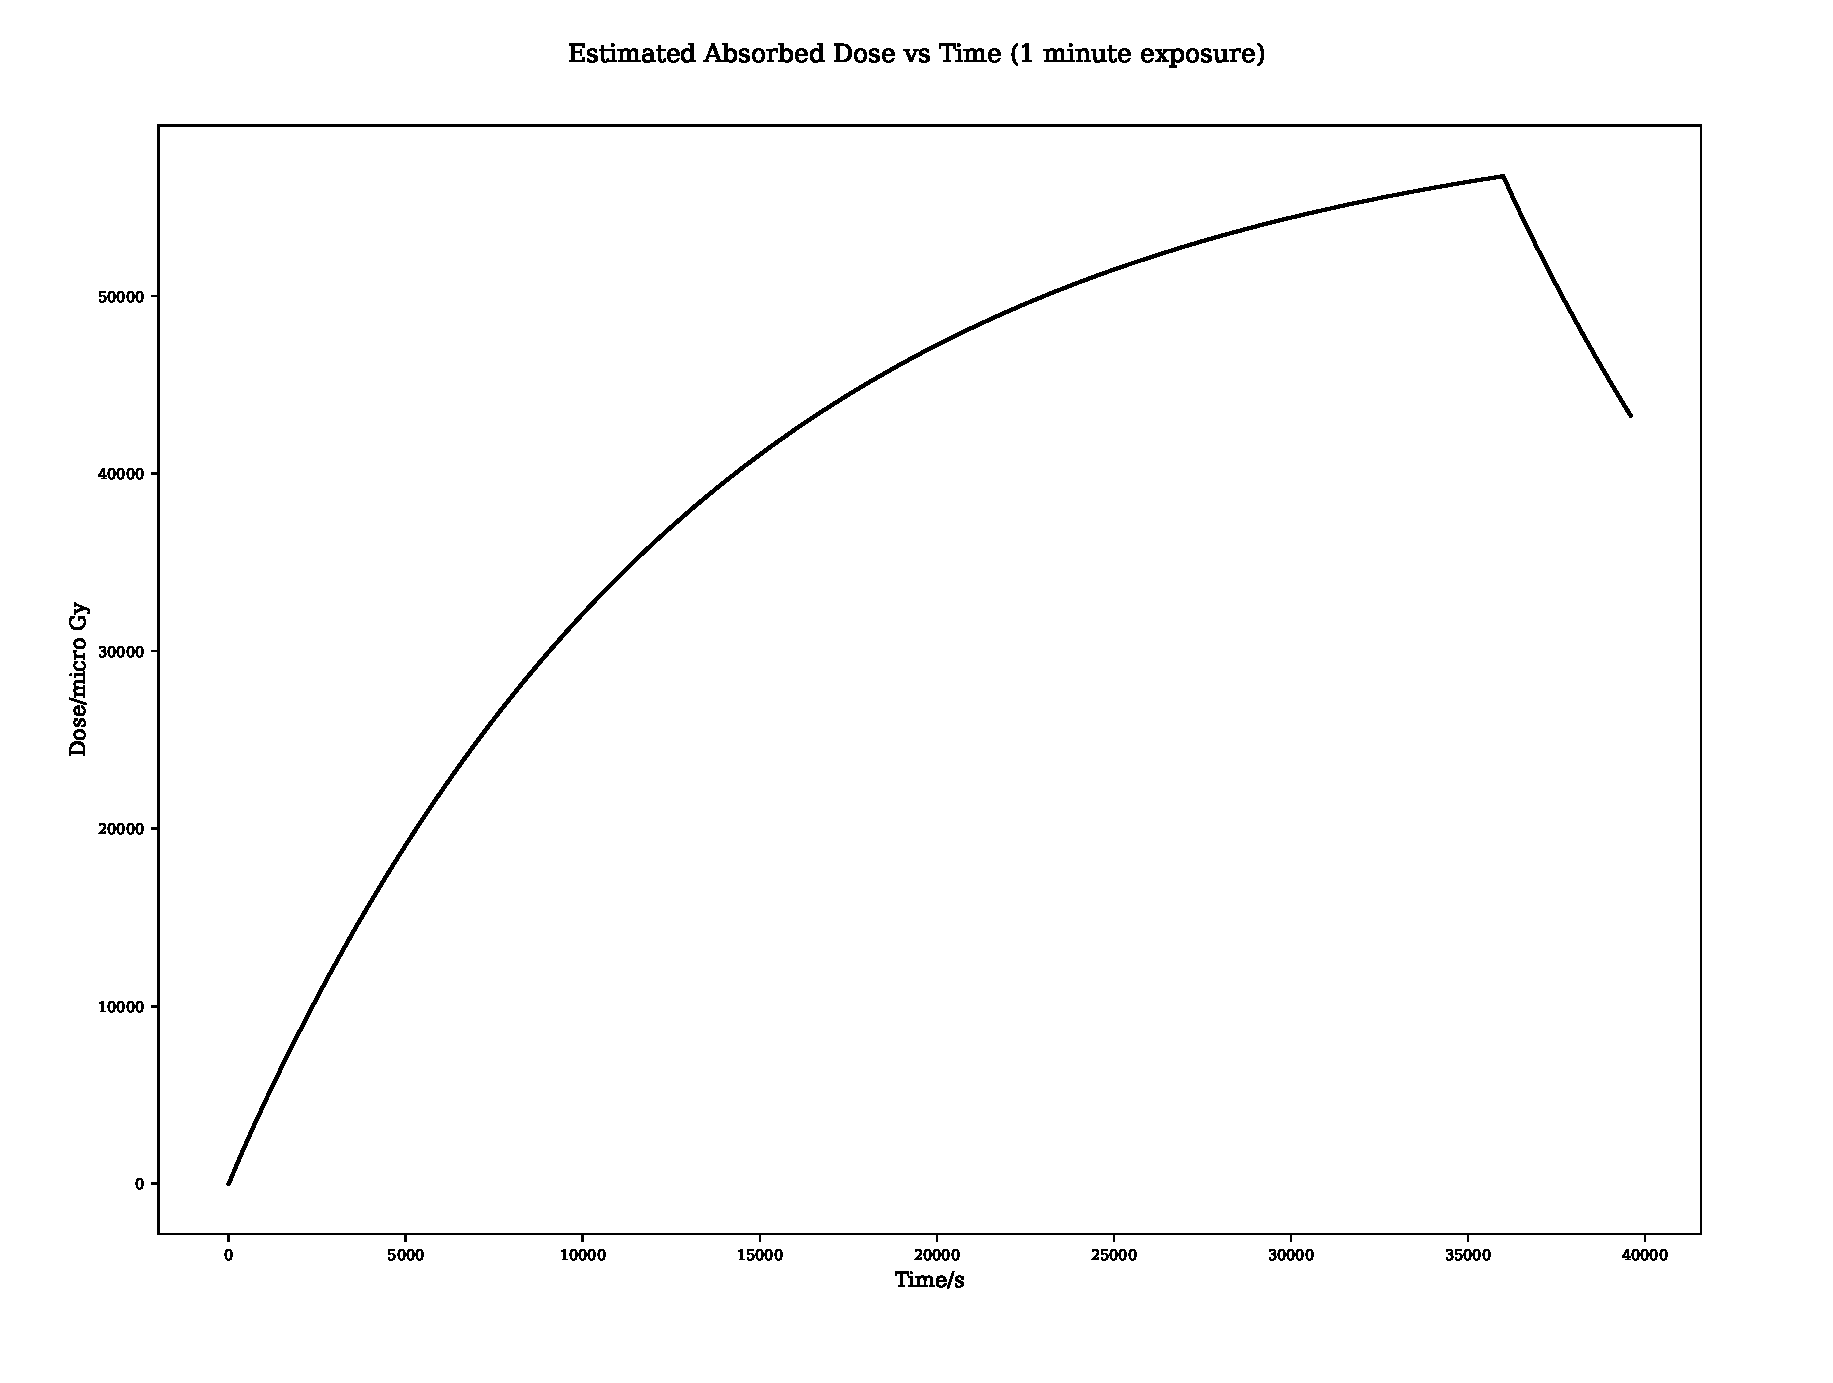
\includegraphics[width=15.0cm]{chapters/background_radiation_effects_and_transport/neutron_plots/2/gamma_dose.eps}
    \captionsetup{font={it}}
    \caption{Steel Irradiation Gamma Dose 1.0e14 Neutrons per cmsquared per second}
    \label{fig:ga_vs_sim_512_2}
  \end{center}
\end{figure}



\subsection{Effect of Radiation on Organics}

Life evolved on Earth from single cell to multicelled organisms such as humans.  Prokaryotic cells are single celled organisms that do not have a nucleus, an example being bacteria.  Our cells are eukarytic cells, and these have a nucleus that contains the genetic information.  Millions of cells die in our body every second, and our body replaces these by replicating living cells.  During the replication stage, the DNA within the nucleus is replicated.    

DNA is a polymer that is carefully constructed from six components.  Stretched out, it is approximately 2m in length and approximately 25 angstrom wide, and it is neatly contained within the cell nucleus which is on average just 6 microns across.  The structure of DNA is the well known double helix.  The sides of the helix are made from alternating sugars and phosphates, while the "rungs" of the ladder like structure are pairs of either thymine and adenine or cytosine and guanine.  These pairs are covelantly bonded to the sugar-phosphate sides, and by hydrogen bonds to each other.

Mitosis is the part of the cell cycle where the DNA within the nucleus is replicated and the cell splits into two.  There are repair mechanisms, but if the DNA beyond repair, the cell may die through apoptosis, or it may replicate in an uncontrolled way leading to cancer.


\subsection{Damage Types}

Direct damage is caused when ionising radiation alters or destroys sections of DNA through a direct collision, for example a neutron colliding with and knocking out an atom in the DNA strand.

Our cells are predominantly water, so there is a higher probability of the radiation colliding with water molecules than DNA directly.  The chemistry of the contents of the cell is changed, for example by the creation of free radicals, and these lead to damage of DNA as an indirect result of radiation passing through the cell.

\subsection{Collision Event}

The damage event in a material such as Steel takes place in stages, and this is similar to the way the event is handled for biological structures.

\begin{figure}[tbp]
\centering
\begin{tikzpicture}[node distance=2cm]
\node (a) [startstop] {Physical stage - picoseconds};
\node (b) [process, below of=a] {Physiochemical};
\node (c) [process, below of=b] {Chemical};
\node (d) [startstop, below of=c] {Biological};
%% arrows
\draw [->] (a) -- (b);
\draw [->] (b) -- (c);
\draw [->] (c) -- (b);
\end{tikzpicture}
\captionsetup{font={it}}
\caption{}
\label{fig:decaychain}
\end{figure}














